%!TEX root = /Users/nebolsin/Documents/MSU/Graduate Work/tex/main.tex
\section{Введение} 
\label{intro}

Целью данной работы является создание распределенной вычислительной среды (РВС), ориентированной на высокоуровневое решение задач. Система упростит доступ ученых и исследователей к вычислительным ресурсам, в частности, к высокопроизводительным суперкомпьютерам факультета ВМиК, таким как BlueGene/P и Regatta. Вычислительная среда позволит, используя веб-интерфейс, как производить рассчеты при помощи предустановленных компонентов (обработка данных), так и создавать новые компоненты и тестировать их на различных конфигурациях высокопроизводительных параллельных систем (исследование параллельных алгоритмов).

В разделах~\ref{intro}--\ref{review} данной работы анализируются основные сценарии работы с вычислительными средами, описывается пять существующих узкоспециализированных систем для решения задач (problem-solving) и показывается необходимость создания РВС, рассчитанной на широкий класс задач. После чего, в разделе~\ref{research} предлагается архитектура построения подобной системы и в разделе~\ref{practical} реализуется рабочий прототип системы, рассчитанный на работу на доступных факультету ВМиК вычислительных мощностях.

Распределенные вычислительные среды  в последние несколько лет приобретают все большую популярность. Основными движущими факторами этого процесса являются улучшения в технологической инфраструре, а также более полное понимание потребностей ученых и инженеров, работающих в прикладных областях. В частности, сдвиг от низкоуровнего запуска и планирования приложений в сторону более высокоуровнего подхода решения проблем показывает, что распределенные вычислительные среды будут приобретать все большую и большую важность в научных исследованиях. В этой работе термин РВС будет использоваться для обозначения в широком смысле любых средств, которые позволяют ученому или инженеру использовать распределенные вычисления для решения вычислительных задач. Это определение, таким образом, включает как высокопроизводительные научные библиотеки, имеющие возможность работать в распределенной (или параллельной) среде, так и предметные среды решения задач (PSE).

РВС расширяет понятие программной среды за рамки парадигмы <<компиляция-планирование-выполнение>> и включает такую функциональность, как доступ по сети, информационные сервисы, работа с данными и совместная работа над задачей. Эта функциональность становится особенно важна для поддержки междисциплинарных научных сообществ. При наблюдениях за работой больших групп ученых и инженеров над большими приложениями (авиационный дизайн, разработка систем беспроводных коммуникаций, и т.д.) были выявлены некоторые \cite{Ramakrishnan02} повторяющиеся ситуации, возникающие при проведении таких исследований.

Далее в этом разделе будут рассмотрены сценарии использования вычислительных сред, которые помогут сформулировать требования к РВС. Также будет описана высокоуровневая структура, необходимая для разработки и организации программных сред, использующихся научными сообществами.

\subsection{Cценарии работы научных сообществ}
\label{scenarios}

Начнем с описания некоторых сценариев, чтобы проиллюстрировать обычные потребности междисциплинарных научных сообществ. Существуют фундаментальные различия в шаблонах использования вычислительных сред между одиночным ученым, работающим над более или менее однородной проблемой и научными сообществами. Например, как проблемы сообщества, решающего задачу вычисления собственных значений матрицы, отличаются от проблем сообщества, занимающегося авиационным моделированием или беспроводными коммуникациями? Выделяются три сценария, которые показывают эти различия.

\textbf{Сценарий 1.} Специалист по трассировке лучей, разработчик каналов связи и программист решают проблему нахождения такого размещения беспроводной базовой станции на квадратном километре большого города, которое будет давать оптимальное покрытие. Эта проблема требует вычислений, которые можно представить как граф из компонентов, написанных на разных языках программирования (C, Matlab, FORTRAN) и работающий в одном большом оптимизационном цикле. На разных стадиях выполнения происходит обмен информацией между компонентами, написанными на разных языках. Дополнительно, получается большое количество промежуточных результатов, не все из которых имеют прямое отношение к решаемой задаче оптимизации. Такие результаты обычно кэшируются для увеличения производительности, могут быть визуализированы на разных стадиях выполнения или просто сохранены для дальшейшего изучения. Более того, компоненты (код) разрабатываются в разное время разными исследователями и многие из них могут находиться в состоянии активной разработки. В этом случае невозможно четко специфицировать форматы ввода-вывода для каждого из компонентов. Кроме того, сама структура связи между компонентами может меняться со временем. Таким образом, программная среда должна позволять соотносить спецификацию задачи с конкретым кодом и иметь возможность произвольно связывать компоненты между собой.

\textbf{Сценарий 2.} Команда авиационных инженеров и специалистов по теории чисел пытаются максимизировать подъемный вес самолета, используя модель, включающую 29 параметров и 68 ограничений. Высококачественный код работает с аэродинамикой, механикой и геометрией определяет, как изменения в параметрах влияют на подъемный вес. В данном приложении предметная область характеризуется не избытком информации, а, наоборот, нехваткой (что вносит свой вклад в стоимость и время проведения имитаций). Следовательно, решение должно сочетать в себе вычисления высокой точности и сложную систему управления данными, которая позволит сконцентрировать усилия по сбору данных на самых важных участках. В результате, проведение исследований может включать запуск высокоточных вычеслений, использование аппроксимаций для предсказания подъемного веса и/или запросы к базе данных для нахождения результатов уже проведенных вычислений. Кроме того, вычислительные ресурсы и хранилища данных могут быть географически разделены. Таким образом, среда должна предоставлять унифицированный доступ к такому разному функционалу и использовать программные абстракции, которые позволят использовать ресурсы максимально эффективно.

\textbf{Сценарий 3.} Группа программистов, ядерных физиков и специалистов по производительности разрабатывают Sweep3D, сложный вычислительный комплекс для рассчетов в области ядерной физики. Они понимают, что эффективная разработка данного приложения требует одновременного проведения аналитического моделирования, запуска имитаций и проведения реальных экспериментов. Они используют метасистемную инфраструктуру для объединения этих различных процессов. Однако они не могут заранее определиться как и в какой последовательности эти процессы выполнять: решение может быть принято только в ходе вычислений. Таким образом, архитектура программной среды должна позволять композиционное моделирование когда информация о выборе компонентов получается в ходе вычислений (а не до их запуска).

\subsection{Ключевые аспекты работы междисципринарных сообществ}
\label{aspects}

Ключевой доминирующей идеей в этих сценариях является \emph{композиционное моделирование}. Эта идея, также, широко применяется в качестве внутреннего аспекта распределенных вычислений. В контексте решения задач, Форбус определяет этот термин как <<объединение представлений различных частей вычислений чтобы создать представление вычисления как целого>>. В данной работе этот термин будет употребляться для описания подхода к решению задач и его использование не будет означать применения конкретных технологий, таких как распределенные объектные компоненты.  Например, ручное перемещение файлов с входными и выходными данными между различными исполняемыми программами может рассматриваться как композиционное моделирование (однако, в очень примитивной форме). Таким образом, компонент может быть любой частью программного обеспечения, отдельным исполняемым файлом, или, даже, набором формул, которые помогают ученому формализовать процесс моделирования вычислений.

Вторым аспектом является совместная работа над проектом. По определению, РВС для распределенного сообщества должна поддерживать работу группы ученых и инженеров, а не только одиночных исследователей. Такие пользователи основываются на коде и данных других пользователей и результаты их работы становятся частью общего результата. Пользователи также активно коммуницируют между собой и могут организовывать свою работу над подзадачами непредсказуемым образом. Им может потребоваться совместная работа в реальном времени над данной имитацией, однако физически они часто находятся в разных местах. Инструменты для совместной работы являются основополагающими для междисциплинарных исследований.

Кроме того, РВС для междисциплинарных сообществ имеет уникальную возможность расширения контекста научных и инженерных приложений. Типичная РВС обычно работает с одной конкретной имитацией в данный момент времени. Контекст, о котором идет речь, может включать предыдущие научные результаты, которые могут быть использованы для улучшения эффективности текущих вычислений (также новых вычислений можно вообще избежать, если требуемый результат уже доступен). Контекст также включает историю предыдущих вычислений и производительности алгоритмов, которая может быть использована для более эффективного распределения ресурсов. 

\subsection{Высокоуровневая архитектура распределенных вычислительных систем}
\label{architecture}

В завершение раздела, определим высокоуровневую архитектуру, которую можно использовать в РВС для междисциплинарных сообществ. На рисунке~\ref{fig:high-architecture} показаны основные слои, которые можно выделить при проектировании. Это не является архитектурой в полном смысле этого слова, так как интерфейсы между слоями не определены. 

\begin{figure}[tbh]
  \centering
    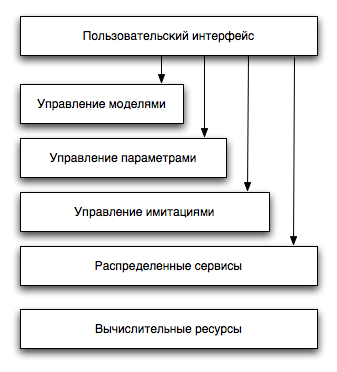
\includegraphics[width=7cm]{images/high-architecture.png}
  \caption{Высокоуровневая архитектура РВС.}
  \label{fig:high-architecture}
\end{figure}  
         
\begin{itemize}
  \item Модель --- это ориентированный граф из исполняемых элементов (компонентов), определяющий поток управления и поток данных в вычислениях. Модель и ее представление в РВС являются различными понятиями. Например, представлением модели в РВС может быть просто имя, а может быть более сложная структура с описанием алгоритмов и принципов работы. Модель состоит из готовых к запуску кусочков кода, которые могут быть параметризованы.
  \item Экземпляр модели --- это модель, для которой заданы все параметры. Иногда параметры могут определяться только в процессе выполнения. 
  \item Имитация --- это экземпляр модели, запущенный на конкретном вычислительном ресурсе. Полезно разделять модель и имитацию, так как, например, один и тот же экземпляр модели может быть запущен на разных вычислительных ресурсах или использовать в работе случайные числа. Каждый из таких запусков будет давать разный результат и по нашему соглашению будет являться отдельной имитацией.
  \item Под распределенными сервисами понимаются любые программные средства, обеспечивающие работу приложения в условиях распределенной среды. Например, подсистема управления данными, позволяющая одному компоненту, запущенному на каком-то вычислительном узле, получить результаты работы другого компонента, работающего на другом вычислительном узле.
\end{itemize}
